\documentclass{beamer}
\usepackage{hyperref}
\title{Cassandra, Hadoop, Pig}
\subtitle{Apache}
\author{Konrad Kurdej}
\date{30-07-2013}
\usetheme{Hannover}

\AtBeginSection[] { 
  \begin{frame}[plain] 
    \tableofcontents[currentsection] 
  \end{frame}
  \addtocounter{framenumber}{-1} 
}

\definecolor{olive}{rgb}{0.3, 0.4, .1}
\definecolor{fore}{RGB}{249,242,215}
\definecolor{back}{RGB}{51,51,51}
\definecolor{title}{RGB}{255,0,90}
\definecolor{dgreen}{rgb}{0.,0.6,0.}
\definecolor{gold}{rgb}{1.,0.84,0.}
\definecolor{JungleGreen}{cmyk}{0.99,0,0.52,0}
\definecolor{BlueGreen}{cmyk}{0.85,0,0.33,0}
\definecolor{RawSienna}{cmyk}{0,0.72,1,0.45}
\definecolor{Magenta}{cmyk}{0,1,0,0}

\begin{document}
\begin{frame}
\titlepage
\end{frame}
\section*{Outline}
\begin{frame}
\tableofcontents
\end{frame}

\section{Cassandra}

\begin{frame}
    \begin{itemize}
        \item implementation of Google's BigTable and Amazon's Dynamo
        \item developed at Facebook
        \item NoSQL - key-value store mixed with columns
        \item no joins or subqueries, emphasizes denormalization
        \item has data structures - list, set, map (64kb limit) - and counters
        \item focused on writes but reads are also fast
    \end{itemize}

\end{frame}


\begin{frame}
\begin{itemize}
 \item used by: Netflix, eBay, Twitter, Reddit, ...
 \item fault tolerant - no single point of failure, replication
 \item performant
 \item decentralized
 \item durable
 \item configurable (for example: (a)sync replication)
 \item scalable \href{http://vldb.org/pvldb/vol5/p1724_tilmannrabl_vldb2012.pdf}{PAPER}
 \item there are companies that provide support
\end{itemize}
\end{frame}


\begin{frame}
    \frametitle{CQL 3 \& Data modeling}
%\href{http://www.datastax.com/documentation/cassandra/1.2/index.html?pagename=docs\&version=1.2\&file=index#cassandra/ddl/ddl_anatomy_table_c.html#concept_ds_qqw_1dy_zj}{example from documentation}
\end{frame}

\section{Hadoop}

\begin{frame}
    \begin{block}{Open-source software for reliable, scalable, distributed computing}
        Modules:
        \begin{description}
            \item[Common] utilities supporting other modules
            \item[HDFS] high-throughput distributed file system
            \item[YARN] framework for job scheduling and resource management
            \item[MapReduce] 
        \end{description}
    \end{block}
\end{frame}


\section{Pig}



\begin{frame}
\begin{center}
\Huge{Q \& m A}

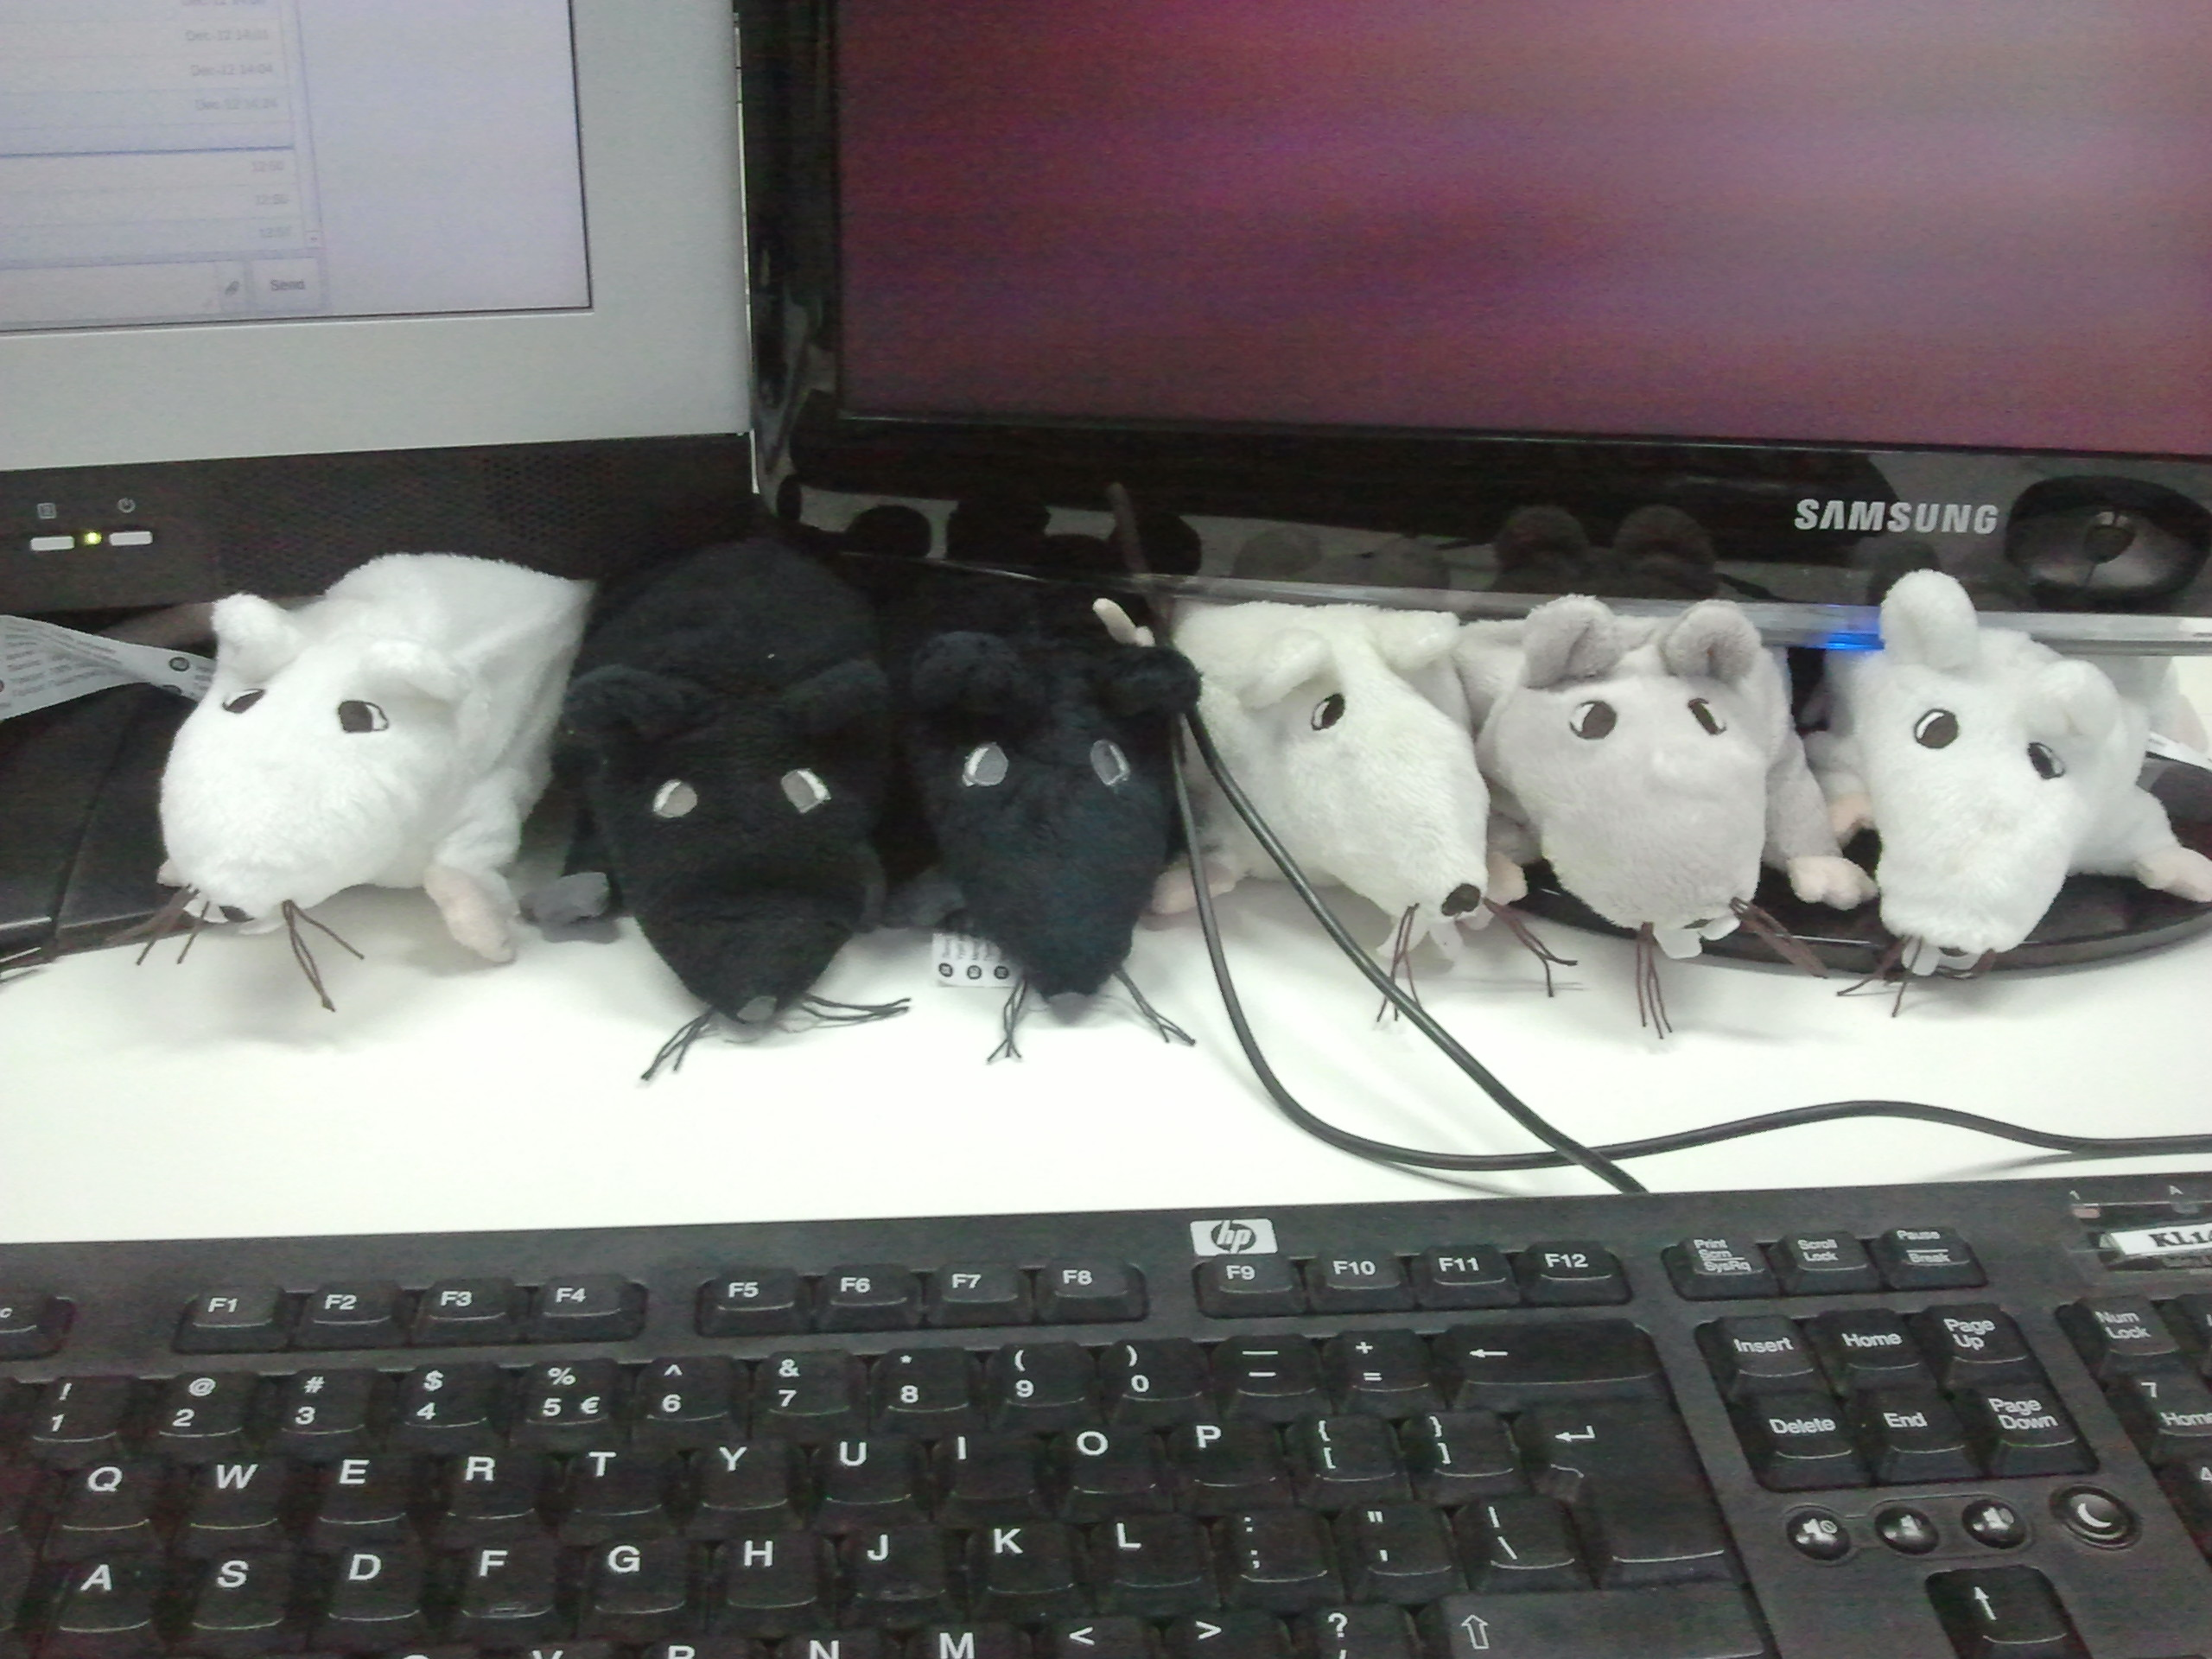
\includegraphics[scale=0.1]{../common/questions.jpg} 

\end{center}

\end{frame}

\end{document}
